%===================================
\subsection{Optimisation Results}

% \begin{figure}[tbh]
%   \centering
% %   \resizebox{5in}{!}{
% %   \turnbox{90}{\small{Rate (sp/s)}}%
% % \includegraphics[keepaspectratio=true,width=0.45\textwidth]{AN_rateplace_10_0.5.eps}\includegraphics[keepaspectratio=true,width=0.45\textwidth]{AN_rateplace_12.5_0.5.eps}\\
% % \includegraphics[keepaspectratio=true,width=0.45\textwidth]{CN_rateplace_10_0.5.eps}\includegraphics[keepaspectratio=true,width=0.45\textwidth]{CN_rateplace_12.5_0.5.eps}
% %   \small{Freq.\ Channel}
% % }
%   \resizebox{5in}{!}{\includegraphics[angle=-90]{NoFigure}}
%   \caption{AN (top) and CN rate-place profiles from the CN stellate model in
%   response to half and 1 octave notch noise inputs. }
%   \label{fig:TVResults}
% \end{figure}

% First Error of 0.0167 (MSE Normalised rate between 4.57--18.68 kHz channels),
% was run in Dec 2009. \yellownote{More work is being done now on a more recent
% result}



% \begin{figure}[h!]
%   \centering
% \resizebox{\textwidth}{!}{\includegraphics{./TV_Notch/spl50/TV_Notch_result.eps}}
%   \caption{Optimisation results for stimulus at 50 dB SPL.  }
%   \label{fig:TV_resultspl50}
% \end{figure}


% \begin{figure}[h!]
%   \centering
% \resizebox{\textwidth}{!}{\includegraphics{./TV_Notch/TV_Notch_result.eps}}
%   \caption{Optimisation results for the reference notch response compressed
%   (lower notch) and expanded (upper notch).}
%   \label{fig:TV_result}
% \end{figure}



Complicated issues in \TV~model optimisation:
\begin{itemize}
\item Input model: reverting back to original Zilany model (2006-2007)
\item Golgi model: from previous tests
\item \DS~model: from previous tests.  Sustained portion does not fire enough even at high notch level (SPL=90).  \TV~response heavily dependant on  \DS~input.
\item \TV~model: Difficult to reconstruct model by changing number or offset during optimisation.
\item \TV~model: \DS2TV connections are STILL randomly selected given number, spread and offset
  \begin{itemize}
  \item connections can be fixed by using mean and Pd, but this discrete method can be crude
  \end{itemize}
\item Experimental data: rate vs notch position is relative to \BF~of unit
\item Experimental data: sound level dependant on \BF~and notch position, this means that the relative spectrum level may be variable along the network
\end{itemize}

% By setting the reversal potential of \TV~cells to $-75$~mV, the optimisation
% produced the following results in Figure~\ref{fig:TV_resultErev75}. In this
% figure, the \TV~rate-place profile gains no benefit from the reduced reversal
% potential.  Some contributing factors that may explain the poor optimisation
% performance are the low firing of \DS~cells and the notch stimulus sound level
% remained at 90 dB \SPL.
% \begin{figure}[h!]
%   \centering
% \resizebox{\textwidth}{!}{\includegraphics{./TV_Notch/Erev-70/TV_Notch_result.eps}}
% \resizebox{\textwidth}{!}{\includegraphics{./TV_Notch/Erev-75/TV_Notch_result.eps}}
%   \caption{Optimisation results for TV Notch model with the reversal potential
%   of TV cells is -75~mV.  }
%   \label{fig:TV_resultErev75}
% \end{figure}

%\smallskip{}

Figure~\ref{fig:TV_result_spl} shows the optimisation results for different input sound intensities.
The performance improves when reducing the sound level of the notch stimulus from 110 down to 50 dB \SPL.

\begin{figure}[htb]
  \centering
  \resizebox{0.6\textwidth}{!}{\includegraphics{./TV_Notch/TV_Notch_spl.eps}}
  \caption[TV cell model: optimisation results]{Optimisation results for TV Notch model with stimulus sound levels at 110, 90, 70 and 50 dB SPL.}
  \label{fig:TV_result_spl}
\end{figure}

% % D~----------------------------------
% \begin{tabularx}{\linewidth}{|X|c|c|c|}
%   \hdr{4}{F}{Optimisation} \\ \hline \textbf{Parameters} & \textbf{Name} &
%   \textbf{Range} & \textbf{Best Values} \\\hline
%   Weight of \DS~syn on \TV~ ($\mu$S)         &    \wDSTV     & [1e-5,0.005]  & 0.0029 \\
%   Weight of \ANF~syn on \TV~ ($\mu$S)         &    \wANFTV    & [1e-5,0.005]  & 0.00017 \\
%   Number of synapses, \LSR~to \TV~          &    \nLSRTV    & [0,64]     & 8           \\
%   Number of synapses, \HSR~to \TV~          &    \nHSRTV    & [0,64]     & 14          \\
%   Spread of \DS~connections onto \TV~(channel units) &    \sDSTV &     [0,10]     & 2.1     \\
%   Offset of \DS~connections onto \TV~(channel units) & \oDSTV & [0,10] & 0.24
%   \\ \hline
% \end{tabularx}

% % D~----------------------------------
% \begin{tabularx}{\linewidth}{|X|c|c|c|}
%   \hdr{4}{F}{Optimisation} \\ \hline \textbf{Parameters} & \textbf{Name} &
%   \textbf{Range} & \textbf{Best Values} \\\hline
%   Number of synapses, \DS~to \TV~  &    \nLSRTV    & [0,300] & 8 \\
%   Number of synapses, \LSR~to \TV~  &    \nLSRTV    & [0,300] & 8 \\
%   Number of synapses, \HSR~to \TV~  &    \nHSRTV    & [0,300] & 14 \\
%   Spread of connections from \DS~onto \TV~(channel units) & \sDSTV & [0,100] & 2.1     \\
%   Offset of \DS~connections onto \TV~(channel units) & \oDSTV & [0,100] & 0.24
%   \\ \hline
% \end{tabularx}



%\subsection{Optimisation }

% Figure~\ref{fig:TV_result_Run1} shows the optimisation results for .
% \begin{figure}[h!]
%   \centering
% \resizebox{\textwidth}{!}{\includegraphics{Run1/spl90/TV_Notch_result.eps}}
% \resizebox{\textwidth}{!}{\includegraphics{Run1/spl50/TV_Notch_result.eps}}
% \resizebox{\textwidth}{!}{\includegraphics{Run1/Erev-70/TV_Notch_result.eps}}
%   \caption{Optimisation results for a refined TV Notch model with stimulus
%   sound levels at 90 and 50 dB SPL and Erev=-70 mV.}
%   \label{fig:TV_result_Run1}
% \end{figure}


To encompass the use of changing the number and spread of synaptic connections a new error function was created to delete all synapses then reconnect the network with the new parameters.
Figure~\ref{fig:TV_result_Run2_50} shows the optimisation results for different input sound intensities.
The performance improves when reducing the sound level of the notch stimulus from 110 down to 50 dB \SPL\@.

\yellownote{TODO: show a simple rate-level plot of HSR, LSR , Golgi, DS, basic TV }

%\smallskip{}

\begin{figure}[htb]
  \centering
  % \resizebox{\textwidth}{!}{\includegraphics{Run2/spl70/TV_Notch_result.eps}}
  \resizebox{\textwidth}{!}{\includegraphics{TV_Notch/Run2/spl50/TV_Notch_result.eps}}
   \caption[Optimisation results for a refined TV cell model]{Optimisation results for a refined TV cell model with stimulus sound levels at 50 dB SPL\@.
The first three runs used the parameters \nDSTV,\wDSTV, \nLSRTV, \nHSRTV, \wLSRTV, \wHSRTV\@.
The second group of 3 runs included the parameters \sDSTV, reversal potential of TV cells, \oDSTV, \nDSTV, \wDSTV.} \label{fig:TV_result_Run2_50}
\end{figure}



% 50 dB Run
{\small%
\noindent%
\begin{center}%table}
%\floatbox{table}[\FBwidth]{%
%\caption{DS cell model optimisation.}\label{tab:DSresults}%
%}%
%\begin{subfloatrow}
%    \subfloat[First optimisation run.]{\label{tab:DSresults:one}%
\begin{minipage}{0.48\linewidth}
\begin{tabularx}{\textwidth}{|X|c|c|c|}
\hdr{4}{}{Optimisation Parameters A} \\ \hline
                &  Run 1  &  Run 2  & Run 3   \\ \hline
    \nDSTV      &   39    &   49    & 59  \\
\wDSTV~($\mu$S) & 0.0217  & 0.0217  & 0.0258  \\
    \nLSRTV     &   21    &   21    & 23  \\
    \nHSRTV     &   15    &   15    & 14  \\
\wLSRTV~($\mu$S)& 0.0069  & 0.0069  & 0.0115  \\
\wHSRTV~($\mu$S)& 0.0013  & 0.0013  & 0.0013  \\ \hline
     Error      & 1255.34 & 1028.70 & 1082.85 \\ \hline
\end{tabularx}%
%}\quad
% \subfloat[Second optimisation run.]{%[Second Table of Results. However, this one has a very long caption that causes problems with alignment.]
%\label{tab:DSresults:two}%
  \end{minipage}\hfill
  \begin{minipage}{0.48\linewidth}
\begin{tabularx}{\textwidth}{|X|c|c|c|}
\hdr{4}{}{Optimisation Parameters B} \\ \hline
                 & Run 1  & Run 2  & Run 3  \\ \hline
\sDSTV~(channel) &  21.3  & 31.31  & 21.31  \\
  \Eleak~(mV)    & -74.96 & -74.96 & -74.96   \\
\oDSTV~(channel) & 22.03  & 22.03  & 22.03  \\
     \nDSTV      &   15   &   15   & 15 \\
\wDSTV~($\mu$S)  & 0.0148 & 0.0148 & 0.0148 \\ \hline
     Error       & 599.37 & 539.1  & 586.74 \\ \hline
\end{tabularx}%
%}
%\end{subfloatrow}
\end{minipage}
\end{center}%table}
}

The first set of parameters (\nDSTV, \wDSTV, \nLSRTV, \nHSRTV, \wLSRTV, \wHSRTV) were run three times to strengthen the validity of the optimisation results.
The obvious outcome from this sets results are the dominance of \LSR~fibre excitatory inputs over \HSR~fibres; and the large counter-balance of \DS~cell inhibition on \TV~cells.
The second set of parameters (\sDSTV, \Eleak \oDSTV, \nDSTV, \wDSTV) were run for an additional three runs to stabilise the \DSTV~parameters.
\nDSTV~and \wDSTV~were included in both sets and showed a large decrease due to the effect of the \TV~cell's leak reversal potential \Eleak scaling down to $-75$~mV\@.

%\smallskip{}

The eventual result of the offset parameter ($\oDSTV = 22.03$) was unexpected.
The offset is equivalent in octaves of 2.5 octaves at the lowest channel to 1.45 at the highest channel.
\citet{ReissYoung:2005} predicted the offset to be 0.3 octaves, which would be between 2 to 4 channels depending on the location in the network.
This is most likely caused by a local minimum in the optimisation and noise in the model prevented the routine from finding lower scores.

%\smallskip{}

Another optimisation run at 70 dB \SPL~produced a better result for the offset parameter and the overall error value of the fitness function.
The offset of \DS~onto \TV~cells was more desirable at 2.1 channels, equivalent to a mean of 0.14 octaves (0.34 octaves at the lowest channel and 0.13 at the highest channel).
The results in the first set (Optimisation A) show the dominance of \LSR~over \HSR~fibres in the number of synapses (29 to 1); and the increased need for \DS~cell inhibition with a high \nDSTV.
% \clearpage \newpage

% 70 dB Run
{\small\noindent%
\begin{center}
  \begin{minipage}[h]{0.48\linewidth}
    \begin{tabularx}{\textwidth}{|X|c|c|c|}
\hdr{4}{}{Optimisation A} \\ \hline
                 & Run 1  & Run 2  & Run 3  \\ \hline
     \nDSTV      &   43   &   23   & 32 \\
\wDSTV~($\mu$S)  & 0.0017 & 0.0017 & 0.0067 \\
    \nLSRTV      &   29   &   32   & 32 \\
    \nHSRTV      &   1    &   1    & 1  \\
\wLSRTV~($\mu$S) & 0.0019 & 0.0019 & 0.0019 \\
\wHSRTV~($\mu$S) & 0.0013 & 0.0013 & 0.0013 \\ \hline
  \hline Error   & 499.20 & 514.86 & 518.54 \\ \hline
\end{tabularx}
  \end{minipage}\hfill
  \begin{minipage}[h]{0.48\linewidth}
    \begin{tabularx}{\textwidth}{|X|c|c|c|}
\hdr{4}{}{Optimisation B} \\ \hline
                 & Run 1  & Run 2  & Run 3  \\ \hline
\sDSTV~(channel) &   13   &   7    & 17 \\
  \Eleak~(mV)    & -65.89 & -67.22 & -67.22 \\
\oDSTV~(channel) &  2.1   &  2.1   & -7.9   \\
     \nDSTV      &   17   &   17   & 16 \\
\wDSTV ($\mu$S)  & 0.0017 & 0.0017 & 0.0017 \\ \hline
  \hline Error   & 435.47 & 457.63 & 492.55 \\ \hline
\end{tabularx}
  \end{minipage}
\end{center}
}


\begin{figure}[htb]
  \centering
%  \resizebox{\textwidth}{!}{\includegraphics{Run2/spl70/TV_Notch_result.eps}}
%  \resizebox{\textwidth}{!}{\includegraphics{Run2/spl50/TV_Notch_result.eps}}
  \caption[Multiple results for a refined TV cell model with stimulus sound   levels at 70 dB SPL]{Optimisation results for a refined TV Notch model with stimulus sound levels at 70 dB SPL\@.
The first three runs used the parameters \nDSTV,\wDSTV, \nLSRTV, \nHSRTV, \wLSRTV, \wHSRTV\@. The second group of 3 runs included the parameters \sDSTV, reversal potential of TV cells, \oDSTV, \nDSTV, \wDSTV.}   \label{fig:TV_result_Run2_70}
\end{figure}

\yellownote{The final error score was best in 70dB runs, but this is not exactly what I wanted. The 22dB in Reiss fit the TV rate-level response around mid way}

%\smallskip{}

The eventual result of the \TV~cell optimisation, highlighted in the following table, was derived from Run 1A and Run 1B in the set using 70 dB \SPL~stimulus.
\yellownote{Explain the table below more. }


{\small%
\noindent%
\begin{tabularx}{\linewidth}{|X|c|c|c|}
\hdr{4}{F}{Optimisation} \\ \hline
                \textbf{Parameters}                  & \textbf{Name} & \textbf{Range}& \textbf{Best Values} \\\hline
       Number of \DS~synapses onto \TV~cells         &    \nDSTV     &    [0,100]    & 17 \\
   Weight of \DS~synapses onto \TV~cells ($\mu$S)    &    \wDSTV     & [1e-5,0.005]  & 0.0029 \\
   Number of synapses, \LSR$\rightarrow$\TV~cells    &    \nLSRTV    &    [0,100]    & 29   \\
   Number of synapses, \HSR$\rightarrow$\TV~cells    &    \nHSRTV    &    [0,100]    & 1  \\
     Weight of \LSR~syn on \TV~cells   ($\mu$S)      &    \wLSRTV    & [1e-5,0.005]  & 0.00017 \\
     Weight of \HSR~syn on \TV~cells   ($\mu$S)      &    \wHSRTV    & [1e-5,0.005]  & 0.00017 \\
 Spread of \DS~connections onto \TV~cells (channel)  &    \sDSTV     &    [0,100]    & 13     \\
 Offset of \DS~connections onto \TV~cells (channel)  &    \oDSTV     &   [-10,30]    & 2.1    \\
Reversal potential of leak current in \TV~cells (mV) &    \Eleak     &   [-80,-50]   & -65.89 \\ \hline
\end{tabularx}
}
\yellownote{Pull everything about the TV cell model together.}

%===================================
\subsection{Verification Results for DS to TV connectivity}


The response of individual type II units to notch and band-pass sweeps in Figure~\ref{fig:TVReissFig9} (reprinted from Figure 9 in \citep*{ReissYoung:2005}) was the main target for the optimisation of \TV~cells.
To replicate the response of a single unit to notch sweeps, notches were generated in GNU~Octave using Chebychev II filters\footnote{\textsf{cheby2} function   in octave-forge signal package.}  with a sampling rate of 100~kHz and an optimal filter number.
The half octave sweep was calculated from -2~to~2~octaves away from 12.7~kHz at 1/32$^{nd}$ increments with logarithmically constant notch widths\footnotemark. A 50 ms stimulus at 50 dB SPL was setup up in the \AN~model for use by the \CN~stellate model.
\footnotetext{Logarithmically constant means the notch width is calculated at
  the centre frequency of the notch and not the \CF~of the unit of interest.}

%\smallskip{}


Figure~\ref{fig:TV_SweepUnit70} shows the response of a unit with similar \CF~(\TV~unit 70, CF=12.76~kHz) to notch and band-pass noise.

\begin{figure}[htb]
%  \centering
  % \resizebox{\textwidth}{!}{\includegraphics{NoFigure}}
  \resizebox{0.8\textwidth}{!}{\includegraphics[height=\textwidth,keepaspectratio,angle=-90]{TV_Notch/BestSweep.eps}}\\
  \resizebox{0.8\textwidth}{!}{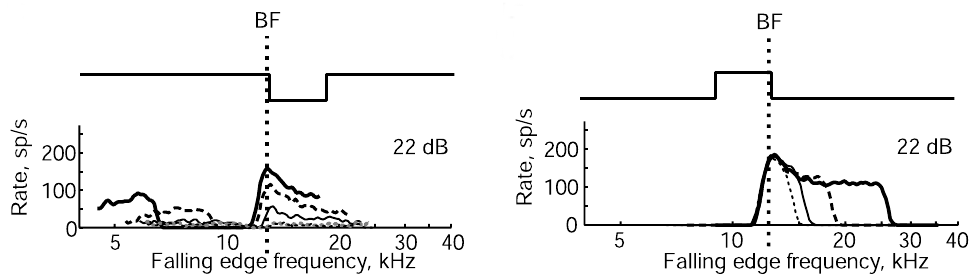
\includegraphics{TV_Notch/Reiss_Fig9_E+F.eps}}\\
  \resizebox{0.8\textwidth}{!}{\includegraphics{TV_Notch/Reiss_Fig10A+B.eps}}\\ \resizebox{0.8\textwidth}{!}{\includegraphics[height=\textwidth,keepaspectratio,angle=-90]{TV_Notch/Best-Offset2/BestSweep.eps}}\\
  \caption[Response of optimised TV cell (CF=12.76~kHz) to notch and band   sweeps]{Response of optimised TV cell (CF=12.76~kHz) to notch and band sweeps with stimulus sound level at 50 dB SPL\@.
Mean rate responses are plotted against the rising edge frequency of the notch and falling edge of the band-pass in octaves relative to 12.7~kHz.
Middle row is from Figure 9 E and F in Reiss and Young, second bottom row is from Figure 10 A and B. }   \label{fig:TV_SweepUnit70}
\end{figure}


The optimised parameters for inputs to the Tuberculoventral cell model were applied to all \TV units across the whole network using tones, noise and tones plus noise stimuli. 
The \TV model outputs' behaviour is shown in Figure~\ref{fig:TV_verification}, similar to the Golgi cell model Figure~\ref{fig:Golgi_verification}. 
Figure~\ref{fig:TV_verification}A and B show the response of the central \TV model (CF=5.8 kHz). The PSTH in Figure~\ref{fig:TV_verification}B is a wide chopper, generated from regular firing type I-c neural model and the strong onset inhibition from DS cells.
%monotonic responses to tones and noise similar to other Ghoshal and Kim units (Figure~\ref{fig:GolgiKimFig2}).  
Figure~\ref{fig:DS_verification}C shows the wide response of all \TV units in the network to a 5.8~kHz tone for increasing sound level. 
The masked response curves (Figure~\ref{fig:DS_verification}D) show the wide-band inhibition particularly for tones above CF. 

\begin{figure}[htb]
%\centering
{\figfont{A}\hspace{0.5\textwidth}\figfont{B}\hfill}\\
%\resizebox{0.95\textwidth}{!}{
\includegraphics[width=0.48\textwidth,keepaspectratio]{ResponsesNoComp/TV_ratelevel_combined.eps}%
\includegraphics[width=0.48\textwidth,keepaspectratio]{ResponsesNoComp/RateLevel/psthsingle50.1.eps}\\
%}\\
{\figfont{C}\hspace{0.5\textwidth}\figfont{D}\hfill}\\
%\resizebox{0.95\textwidth}{!}{
\includegraphics[width=0.48\textwidth,keepaspectratio]{ResponsesNoComp/RateLevel/response_area.1.eps}%
\includegraphics[width=0.48\textwidth,keepaspectratio]{ResponsesNoComp/MaskedResponseCurve3/30/TV_masked.eps}\\
%}\\
% }}
%\resizebox{0.45\textwidth}{!}{\includegraphics{ResponsesNoComp/RateLevel/psthsingle90.3.eps}}\\
%\resizebox{0.45\textwidth}{!}{\includegraphics{ResponsesNoComp/RateLevel/psthsingle50.3.eps}}\\
\caption[Optimised TV cell model responses]{Response of optimised TV cell model at the centre of the network (CF=5.8~kHz). A. Rate level responses to tone, noise and tone plus noise. 
B. Wide chopping PSTH at 50 dB~SPL.  
C. Response area equivalent using all TV units in the network. 
D. Masked response across the CF of the central unit (30 dB noise).} \label{fig:TV_verification}
\end{figure}



% \begin{figure}[h!]
%   \centering
% %   \resizebox{\textwidth}{!}{\includegraphics{NoFigure}}
% \resizebox{\textwidth}{!}{\includegraphics[height=\textwidth,keepaspectratio,angle=-90]{./TV_Notch/Best-Offset2/BestSweep.eps}}\\
%   \caption{Response of TV cell (CF=12.76~kHz, with optimised parameters except
%   offset) and DS cell to half octave notch and band sweeps with stimulus sound
%   level at 50 dB SPL\@. Mean rate responses are plotted against the rising
%   edge frequency of the notch and falling edge of the band-pass in octaves
%   relative to 12.7~kHz.}
%   \label{fig:TV_SweepUnit}
% \end{figure}


% \subsection{Tone Response}
% \begin{figure}[h!]
%   \centering\resizebox{0.95\textwidth}{!}{%
%   \includegraphics{RateLevel/psthsingle90.1.eps}%
%   \includegraphics{RateLevel/TV_ratelevel.eps}}
% \end{figure}
% \begin{figure}[h!]
%   \centering\resizebox{0.95\textwidth}{!}{%
%   \includegraphics{RateLevel/response_area.1.eps}%
%   \includegraphics{RateLevel/response_area_log2.1.eps}}
% \end{figure}
% \begin{figure}[h!]
%   \centering\resizebox{0.95\textwidth}{!}{%
% %   \includegraphics{RateLevel/response_area.1.eps}
%   \includegraphics{RateLevel/psthall90.1.eps}%
%   \includegraphics{RateLevel/psthVlevel.1.eps}}
% \end{figure}


% \clearpage
% \subsection{Noise Response}
% \begin{figure}[h!]
%   \centering\resizebox{0.95\textwidth}{!}{%
%   \includegraphics{NoiseRateLevel/psthsingle120.1.eps}%
%   \includegraphics{NoiseRateLevel/TV_ratelevel.eps}}
% \end{figure}
% \begin{figure}[h!]
%   \centering\resizebox{0.95\textwidth}{!}{%
%   \includegraphics{NoiseRateLevel/response_area.1.eps}%
%   \includegraphics{NoiseRateLevel/response_area_log2.1.eps}}
% \end{figure}
% \begin{figure}[h!]
%   \centering\resizebox{0.95\textwidth}{!}{%
% %   \includegraphics{RateLevel/response_area.1.eps}
%   \includegraphics{NoiseRateLevel/psthall90.1.eps}%
%   \includegraphics{NoiseRateLevel/psthVlevel.1.eps}}
% \end{figure}


% \clearpage
% \subsection{Masked Noise and Tone}
% \begin{figure}[h!]
% \centering\resizebox{0.95\textwidth}{!}{\includegraphics{MaskedRateLevel/psthsingle90.1.eps}\includegraphics{MaskedRateLevel/TV_ratelevel.eps}}
% \end{figure}
% \begin{figure}[h!]
%   \centering\resizebox{0.95\textwidth}{!}{%
%   \includegraphics{MaskedRateLevel/response_area.1.eps}%
%   \includegraphics{MaskedRateLevel/response_area_log2.1.eps}}
% \end{figure}
% \begin{figure}[h!]
%   \centering\resizebox{0.95\textwidth}{!}{%
% %   \includegraphics{RateLevel/response_area.1.eps}
%   \includegraphics{MaskedRateLevel/psthall90.1.eps}%
%   \includegraphics{MaskedRateLevel/psthVlevel.1.eps}}
% \end{figure}
% \clearpage
% \subsection{Masked Response Area}
% \begin{figure}[h!]
%   \centering\resizebox{0.95\textwidth}{!}{%
%   \includegraphics{MaskedResponseCurve/psthsingle5810.1.eps}%
%   \includegraphics{MaskedResponseCurve/TV_masked.eps}}
% \end{figure}
% \begin{figure}[h!]
%   \centering\resizebox{0.95\textwidth}{!}{%
%   \includegraphics{MaskedResponseCurve/response_area.1.eps}%
% \includegraphics{MaskedResponseCurve/response_area_log2log2.1.eps}}
% \end{figure}
% \begin{figure}[h!]
%   \centering\resizebox{0.95\textwidth}{!}{%
% %   \includegraphics{RateLevel/response_area.1.eps}
%   \includegraphics{MaskedResponseCurve/psthall5810.1.eps}%
%   \includegraphics{MaskedResponseCurve/psthVmod.1.eps}}
% \end{figure}
% \clearpage





%%% Local Variables:
%%% mode: latex
%%% mode: tex-fold
%%% mode: visual-line
%%% TeX-master: "SimpleResponses"
%%% TeX-PDF-mode: nil
%%% End:
